\documentclass[a4paper]{article}
\usepackage{xcolor}
\usepackage{listings}

\colorlet{mygray}{black!30}
\colorlet{mygreen}{green!60!blue}
\colorlet{mymauve}{red!60!blue}

\lstset{
  backgroundcolor=\color{gray!10},  
  basicstyle=\ttfamily,
  columns=fullflexible,
  breakatwhitespace=false,      
  breaklines=true,                
  captionpos=b,                    
  commentstyle=\color{mygreen}, 
  extendedchars=true,              
  frame=single,                   
  keepspaces=true,             
  keywordstyle=\color{blue},      
  language=c++,                 
  numbers=none,                
  numbersep=5pt,                   
  numberstyle=\tiny\color{blue}, 
  rulecolor=\color{mygray},        
  showspaces=false,               
  showtabs=false,                 
  stepnumber=5,                  
  stringstyle=\color{mymauve},    
  tabsize=3,                      
  title=\lstname                
}
\usepackage[pdftex,
            pdfauthor={NGUYEN MINH HUNG},
            pdftitle={The Title},
            pdfsubject={OPERATING SYSTEM},
            pdfkeywords={Some Keywords},
            pdfproducer={Latex with hyperref, or other system},
            pdfcreator={pdflatex, or other tool}]{hyperref}
\usepackage{a4wide,amssymb,epsfig,latexsym,multicol,array,hhline,fancyhdr}
\usepackage{vntex}
\usepackage{amsmath}
\usepackage{lastpage}
\usepackage[lined,boxed,commentsnumbered]{algorithm2e}
\usepackage{enumerate}
\usepackage{color}
\usepackage{graphicx}							% Standard graphics package
\usepackage{array}
\usepackage{tabularx, caption}
\usepackage{multirow}
\usepackage{multicol}
\usepackage{rotating}
\usepackage{graphics}
\usepackage{geometry}
\usepackage{setspace}
\usepackage{epsfig}
\usepackage{tikz}
\usetikzlibrary{arrows,snakes,backgrounds}
\usepackage{hyperref}
\hypersetup{urlcolor=blue,linkcolor=black,citecolor=black,colorlinks=true} 
%\usepackage{pstcol} 								% PSTricks with the standard color package

\newtheorem{theorem}{{\bf Theorem}}
\newtheorem{property}{{\bf Property}}
\newtheorem{proposition}{{\bf Proposition}}
\newtheorem{corollary}[proposition]{{\bf Corollary}}
\newtheorem{lemma}[proposition]{{\bf Lemma}}

\AtBeginDocument{\renewcommand*\contentsname{Contents}}
\AtBeginDocument{\renewcommand*\refname{References}}
%\usepackage{fancyhdr}
\setlength{\headheight}{40pt}
\pagestyle{fancy}
\fancyhead{} % clear all header fields
\fancyhead[L]{
 \begin{tabular}{rl}
    \begin{picture}(25,15)(0,0)
    \put(0,-8){
\includegraphics[width=8mm, height=8mm]{hcmut.png}}
    %\put(0,-8){\epsfig{width=10mm,figure=hcmut.eps}}
   \end{picture}&
	%
\includegraphics[width=8mm, height=8mm]{hcmut.png} & %
	\begin{tabular}{l}
		\textbf{\bf \ttfamily University of Technology, Ho Chi Minh City}\\
		\textbf{\bf \ttfamily Faculty of Computer Science and Engineering}
	\end{tabular} 	
 \end{tabular}
}
\fancyhead[R]{
	\begin{tabular}{l}
		\tiny \bf \\
		\tiny \bf 
	\end{tabular}  }
\fancyfoot{} % clear all footer fields
\fancyfoot[L]{\scriptsize \ttfamily Assignment for Operating System - Academic year 2020 - 2021}
\fancyfoot[R]{\scriptsize \ttfamily Page {\thepage}/\pageref{LastPage}}
\renewcommand{\headrulewidth}{0.3pt}
\renewcommand{\footrulewidth}{0.3pt}


%%%
\setcounter{secnumdepth}{4}
\setcounter{tocdepth}{3}
\makeatletter
\newcounter {subsubsubsection}[subsubsection]
\renewcommand\thesubsubsubsection{\thesubsubsection .\@alph\c@subsubsubsection}
\newcommand\subsubsubsection{\@startsection{subsubsubsection}{4}{\z@}%
                                     {-3.25ex\@plus -1ex \@minus -.2ex}%
                                     {1.5ex \@plus .2ex}%
                                     {\normalfont\normalsize\bfseries}}
\newcommand*\l@subsubsubsection{\@dottedtocline{3}{10.0em}{4.1em}}
\newcommand*{\subsubsubsectionmark}[1]{}
\makeatother


\begin{document}

\begin{titlepage}
\begin{center}
VIETNAM NATIONAL UNIVERSITY, HO CHI MINH CITY \\
UNIVERSITY OF TECHNOLOGY \\
FACULTY OF COMPUTER SCIENCE AND ENGINEERING
\end{center}

\vspace{1cm}

\begin{figure}[h!]
\begin{center}

\includegraphics[width=3cm]{hcmut.png}
\end{center}
\end{figure}

\vspace{1cm}


\begin{center}
\begin{tabular}{c}
\multicolumn{1}{l}{\textbf{{\Large OPERATING SYSTEMS (CO2017)}}}\\
~~\\
\hline
\\
\multicolumn{1}{l}{\textbf{{\Large Assignment}}}\\
\\
\textbf{{\Huge Simple Operating System}}\\
\\

\\
\hline
\end{tabular}
\end{center}

\vspace{3cm}

\begin{table}[h]
\begin{tabular}{rrl}
\hspace{5 cm} & Advisor: & Nguyễn Lê Duy Lai\\
& Students: & Nguyễn Minh Hùng - 1952737 \\
& & Phạm Nhật Hoàng - 1952703 \\
& & Bùi Quang Tiến - 1953018
 \\
\end{tabular}
\end{table}

\begin{center}
{\footnotesize HO CHI MINH CITY, SEPTEMBER 2021}
\end{center}
\end{titlepage}


%\thispagestyle{empty}

\newpage
\tableofcontents
\newpage


%%%%%%%%%%%%%%%%%%%%%%%%%%%%%%%%%

%%%%%%%%%%%%%%%%%%%%%%%%%%%%%%%%%
\section{Scheduler}
    \\
	\subsection{Scheduling algorithms (Priority Feedback Queue)}
	\hfill\\
	{\bfseries QUESTION}: What is the advantage of using priority feedback queue in comparison with other scheduling algorithms you have learned?\\
	\\
	\textbf{Solution} \\
	\\
	The \textbf{Priority Feedback Queue} has a number of \textbf{distinct queues}, each
    assigned a \textbf{different priority level}. It allows
    a process to move between queues. Also, it uses the ideas of other scheduling algorithms we have learned for each queue such as: First Come First Served (FCFS), Round Robin (RR), Priority Scheduling (PS),  Multilevel Feedback Queue, etc...\\
    \\
    The following algorithms are what we have learned:\\
    \begin{itemize}
        \item First Come First Served (FCFS)
        \item Shortest Job First (SJF)
        \item Shortest Remaining Time First (SRTF)
        \item Priority Scheduling (PS)
        \item Round Robin (RR)
        \item Multilevel Queue Scheduling (MLQS)
        \item Multilevel Feedback Queue (MLFQ)
    \end{itemize}

    In this assignment, we implemented 2 queues \texttt{ready\_queue} and
    \texttt{run\_queue} as follows: \\
    \begin{itemize}
    \item \texttt{ready\_queue}: storing processes with assigned priority and the important point is that this has higher priority than \texttt{run\_queue}'s. \\
    \item \texttt{run\_queue}: storing processes that are wating to execute. In case \texttt{ready\_queue} is empty, we push all into \texttt{ready\_queue} to continue paused processes. \\
    \end{itemize}
    These two queues are both \textbf{Priority Queues}, the assigned priority are given depending on process characteristics. \\
    \\
    Compared to others, PFQ has some advantages as follows: \\
    \begin{itemize}
        \item The CPU runs processes in \textbf{round-robin} style. Every process gets an equal share of the CPU. RR is cyclic in nature, so there is \textbf{no starvation}.
        \item Using 2 priority queues with each assigned priority processes, it is based on MLQS and MLFQ. The processes are permanently assigned to the queue, so it has advantage of low scheduling overhead, moreover, it prevents starvation by moving a process that waits too long for lower priority queue (\texttt{run\_queue}) to the higher priority queue (\texttt{ready\_queue}). 
    \end{itemize}
	\subsection{Gantt diagrams results}
	\hfill \\
	{\bfseries REQUIREMENT: }Draw Gantt diagram describing how processes are executed by the CPU.\\
	\begin{figure}[h]
	    \centering
	    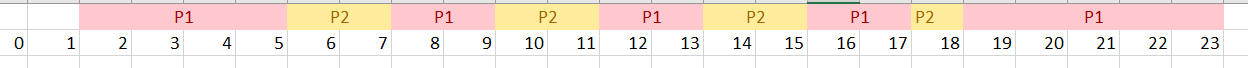
\includegraphics[width=\textwidth]{TEST0.PNG}
	    \caption{Gantt chart for processes in test sched\_0}
	    \label{fig:my_label}
	\end{figure}
	
	\begin{figure}[h]
	    \centering
	    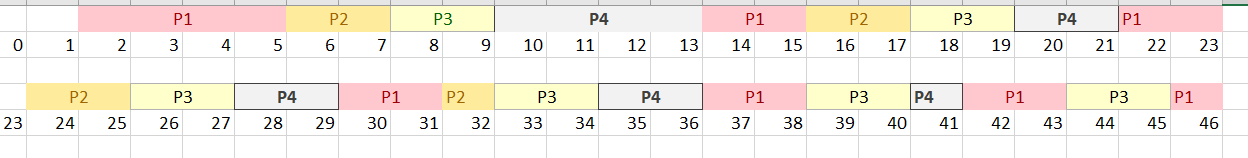
\includegraphics[width=\textwidth]{TEST1.PNG}
	    \caption{Gantt chart for processes in test sched\_1}
	    \label{fig:my_label}
	\end{figure}
    You can also see the result in \texttt{my\_output/sched.txt} \\
    \newpage
	\subsection{Implementation}
	\subsubsection{Priority queue}
	\hfill\\
	The \textbf{Priority Queue} accepts the following properties:
	\begin{itemize}
	    \item Every item has a priority associated with it.
        \item An element with high priority is dequeued before an element  with low priority.
        \item If two elements have the same priority, they are served according to their order in the queue.
	\end{itemize}
	In this assignment, we simplify it by implementing \textbf{ArrayQueue}
	with \texttt{MAX\_QUEUE\_SIZE} = 10 , as follows:
	\begin{itemize}
	    \item \texttt{enqueue()} : just simply add to the end of array in O(1) time.
	    \item \texttt{dequeue()} : linearly searching an item with highest priority, then removing the item by moving all subsequent items one position back.
	\end{itemize}
	The following is the implementation of \texttt{queue.c} \\

	\begin{lstlisting}
    void enqueue(struct queue_t * q, struct pcb_t * proc) {
    	/* TODO: put a new process to queue [q] */
    	if (q->size == MAX_QUEUE_SIZE) return;
    	q->proc[q->size++] = proc;
    }
    
    struct pcb_t * dequeue(struct queue_t * q) {
    	/* TODO: return a pcb whose prioprity is the highest
    	 * in the queue [q] and remember to remove it from q
    	 * */
    	if (q->size == 0) return NULL;  // if queue size = 0, do nothing
    	int highest_priority_idx = 0, j;
    	for (j = 1; j < q->size; j++) { // traverse to find highest prior. index
     		if (q->proc[j]->priority < q->proc[highest_priority_idx]->priority) {
    			highest_priority_idx = j;
    		}
    	}
    	struct pcb_t * res = q->proc[highest_priority_idx]; // get it out
    	for (j = highest_priority_idx+1; j < q->size; j++) {
    		q->proc[j-1] = q->proc[j]; // shift back to rearrange the queue
    	}
    	q->size--;
    
    	return res;
    }
	\end{lstlisting}
	\subsubsection{Scheduler}
	\hfill\\
	The task of \textbf{scheduler} is to manage and update new process (in \texttt{loader()} function) which is described in Figure 2. However, in this assignment, we just need to complete finding a process for CPU with 2 available queues.
	\begin{itemize}
	    \item \texttt{get\_proc()}: return the process in \texttt{ready\_queue}, if the queue is empty, we push all processes from \texttt{run\_queue}. Then, if we continue to \texttt{dequeue} and get the highest priority process from \texttt{ready\_queue}.
	\end{itemize}
	\hfill \\
	The following is the implementation of \texttt{sched.c} : \\
	
	\begin{lstlisting}
    struct pcb_t * get_proc(void) {
    	struct pcb_t * proc = NULL;
    	/* 
    	 * TODO: get a process from [ready_queue]. 
    	 * If ready queue is empty, 
    	 * push all processes in [run_queue] back to [ready_queue] 
    	 * and return the highest priority one.
    	 * Remember to use lock to protect the queue.
    	 */
    
    	pthread_mutex_lock(&queue_lock);
    	if (empty(&ready_queue)) {
    		// move all process is waiting in run_queue back to ready_queue
    		while (!empty(&run_queue)) {
    			enqueue(&ready_queue, dequeue(&run_queue));
    		}
    	}
    
    	if (!empty(&ready_queue)) {
    		proc = dequeue(&ready_queue);
    	}
    	pthread_mutex_unlock(&queue_lock);
    
    	return proc;
    }
	\end{lstlisting}
	\newpage 
%%%%%%%%%%%%%%%%%%%%%%%%%%%%%%%%%
\section{Memory management}
	\subsection{Segmentation with Paging}
	\hfill\\
	{\bfseries QUESTION:} What is the advantage and disadvantage of segmentation with paging ? \\
	\\
	{\bfseries Solution}\\
	\\
	In \textbf{Segmentation with Paging}, the main memory is divided into variable size segments which are further divided into fixed size pages.\\
    \begin{itemize}
        \item Pages are smaller than segments.
        \item Each Segment has a page table which means every program has multiple page tables.
        \item The logical address is represented as \textbf{Segment Number (base address), Page number and page offset.}
    \end{itemize}
    \hfill\\
    {\large {\bfseries Advantages of Segmentation with Paging}}
    \begin{itemize}
        \item It reduces memory usage.
        \item Page table size is limited by the segment size.
        \item Segment table has only one entry corresponding to one actual segment.
        \item External Fragmentation is not there.
        \item It simplifies memory allocation.
    \end{itemize}
    \hfill \\
    {\large {\bfseries Disadvantages of Segmentation with Paging}}
    \begin{itemize}
        \item Internal Fragmentation will be there.
        \item The complexity level will be much higher as compare to paging.
        \item Page Tables need to be contiguously stored in the memory.
    \end{itemize}
    \hfill\\
	\subsection{Memory status results (RAM)}
	\hfill\\
	\textbf{REQUIREMENT}: Show the status of RAM after each memory allocation and deallocation function call.\\
	\\
	\\
	The following result illustrates \testbf {MEM\_STAT} after each \textbf{allocation and deallocation} function call. \\
	\newpage
	{\bfseries TEST 0} \\
	
	\begin{lstlisting}
    ------ MEMORY MANAGEMENT TEST 0 --------------
    ./mem input/proc/m0
    ----------------ALLOCATION--------------------

    000: 00000-003ff - PID: 01 (idx 000, nxt: 001)
    001: 00400-007ff - PID: 01 (idx 001, nxt: 002)
    002: 00800-00bff - PID: 01 (idx 002, nxt: 003)  
    003: 00c00-00fff - PID: 01 (idx 003, nxt: 004)
    004: 01000-013ff - PID: 01 (idx 004, nxt: 005)
    005: 01400-017ff - PID: 01 (idx 005, nxt: 006)
    006: 01800-01bff - PID: 01 (idx 006, nxt: 007)
    007: 01c00-01fff - PID: 01 (idx 007, nxt: 008)
    008: 02000-023ff - PID: 01 (idx 008, nxt: 009)
    009: 02400-027ff - PID: 01 (idx 009, nxt: 010)
    010: 02800-02bff - PID: 01 (idx 010, nxt: 011)
    011: 02c00-02fff - PID: 01 (idx 011, nxt: 012)
    012: 03000-033ff - PID: 01 (idx 012, nxt: 013)
    013: 03400-037ff - PID: 01 (idx 013, nxt: -01)
    ----------------ALLOCATION--------------------

    000: 00000-003ff - PID: 01 (idx 000, nxt: 001)
    001: 00400-007ff - PID: 01 (idx 001, nxt: 002)
    002: 00800-00bff - PID: 01 (idx 002, nxt: 003)
    003: 00c00-00fff - PID: 01 (idx 003, nxt: 004)
    004: 01000-013ff - PID: 01 (idx 004, nxt: 005)
    005: 01400-017ff - PID: 01 (idx 005, nxt: 006)
    006: 01800-01bff - PID: 01 (idx 006, nxt: 007)
    007: 01c00-01fff - PID: 01 (idx 007, nxt: 008)
    008: 02000-023ff - PID: 01 (idx 008, nxt: 009)
    009: 02400-027ff - PID: 01 (idx 009, nxt: 010)
    010: 02800-02bff - PID: 01 (idx 010, nxt: 011)
    011: 02c00-02fff - PID: 01 (idx 011, nxt: 012)
    012: 03000-033ff - PID: 01 (idx 012, nxt: 013)
    013: 03400-037ff - PID: 01 (idx 013, nxt: -01)
    014: 03800-03bff - PID: 01 (idx 000, nxt: 015)
    015: 03c00-03fff - PID: 01 (idx 001, nxt: -01)
    ---------------DEALLOCATION-------------------
    
    014: 03800-03bff - PID: 01 (idx 000, nxt: 015)
    015: 03c00-03fff - PID: 01 (idx 001, nxt: -01)
    ----------------ALLOCATION--------------------
    
    000: 00000-003ff - PID: 01 (idx 000, nxt: 001)
    001: 00400-007ff - PID: 01 (idx 001, nxt: -01)
    014: 03800-03bff - PID: 01 (idx 000, nxt: 015)
    015: 03c00-03fff - PID: 01 (idx 001, nxt: -01)
    ----------------ALLOCATION--------------------
    
    000: 00000-003ff - PID: 01 (idx 000, nxt: 001)
    001: 00400-007ff - PID: 01 (idx 001, nxt: -01)
    002: 00800-00bff - PID: 01 (idx 000, nxt: 003)
    003: 00c00-00fff - PID: 01 (idx 001, nxt: 004)
    004: 01000-013ff - PID: 01 (idx 002, nxt: 005)
    005: 01400-017ff - PID: 01 (idx 003, nxt: 006)
    006: 01800-01bff - PID: 01 (idx 004, nxt: -01)
    014: 03800-03bff - PID: 01 (idx 000, nxt: 015)
    015: 03c00-03fff - PID: 01 (idx 001, nxt: -01)
    Final MEM stat: 
    
    000: 00000-003ff - PID: 01 (idx 000, nxt: 001)
    	003e8: 15
    001: 00400-007ff - PID: 01 (idx 001, nxt: -01)
    002: 00800-00bff - PID: 01 (idx 000, nxt: 003)
    003: 00c00-00fff - PID: 01 (idx 001, nxt: 004)
    004: 01000-013ff - PID: 01 (idx 002, nxt: 005)
    005: 01400-017ff - PID: 01 (idx 003, nxt: 006)
    006: 01800-01bff - PID: 01 (idx 004, nxt: -01)
    014: 03800-03bff - PID: 01 (idx 000, nxt: 015)
    	03814: 66
    015: 03c00-03fff - PID: 01 (idx 001, nxt: -01)
    NOTE: Read file output/m0 to verify your result
    \end{lstlisting}
    \\
    {\bfseries TEST 1}: \\
    \begin{lstlisting}
    ------ MEMORY MANAGEMENT TEST 1 --------------
    ./mem input/proc/m1
    ----------------ALLOCATION--------------------
    
    000: 00000-003ff - PID: 01 (idx 000, nxt: 001)
    001: 00400-007ff - PID: 01 (idx 001, nxt: 002)
    002: 00800-00bff - PID: 01 (idx 002, nxt: 003)
    003: 00c00-00fff - PID: 01 (idx 003, nxt: 004)
    004: 01000-013ff - PID: 01 (idx 004, nxt: 005)
    005: 01400-017ff - PID: 01 (idx 005, nxt: 006)
    006: 01800-01bff - PID: 01 (idx 006, nxt: 007)
    007: 01c00-01fff - PID: 01 (idx 007, nxt: 008)
    008: 02000-023ff - PID: 01 (idx 008, nxt: 009)
    009: 02400-027ff - PID: 01 (idx 009, nxt: 010)
    010: 02800-02bff - PID: 01 (idx 010, nxt: 011)
    011: 02c00-02fff - PID: 01 (idx 011, nxt: 012)
    012: 03000-033ff - PID: 01 (idx 012, nxt: 013)
    013: 03400-037ff - PID: 01 (idx 013, nxt: -01)
    ----------------ALLOCATION--------------------
    
    000: 00000-003ff - PID: 01 (idx 000, nxt: 001)
    001: 00400-007ff - PID: 01 (idx 001, nxt: 002)
    002: 00800-00bff - PID: 01 (idx 002, nxt: 003)
    003: 00c00-00fff - PID: 01 (idx 003, nxt: 004)
    004: 01000-013ff - PID: 01 (idx 004, nxt: 005)
    005: 01400-017ff - PID: 01 (idx 005, nxt: 006)
    006: 01800-01bff - PID: 01 (idx 006, nxt: 007)
    007: 01c00-01fff - PID: 01 (idx 007, nxt: 008)
    008: 02000-023ff - PID: 01 (idx 008, nxt: 009)
    009: 02400-027ff - PID: 01 (idx 009, nxt: 010)
    010: 02800-02bff - PID: 01 (idx 010, nxt: 011)
    011: 02c00-02fff - PID: 01 (idx 011, nxt: 012)
    012: 03000-033ff - PID: 01 (idx 012, nxt: 013)
    013: 03400-037ff - PID: 01 (idx 013, nxt: -01)
    014: 03800-03bff - PID: 01 (idx 000, nxt: 015)
    015: 03c00-03fff - PID: 01 (idx 001, nxt: -01)
    ---------------DEALLOCATION-------------------
    
    014: 03800-03bff - PID: 01 (idx 000, nxt: 015)
    015: 03c00-03fff - PID: 01 (idx 001, nxt: -01)
    ----------------ALLOCATION--------------------
    
    000: 00000-003ff - PID: 01 (idx 000, nxt: 001)
    001: 00400-007ff - PID: 01 (idx 001, nxt: -01)
    014: 03800-03bff - PID: 01 (idx 000, nxt: 015)
    015: 03c00-03fff - PID: 01 (idx 001, nxt: -01)
    ----------------ALLOCATION--------------------
    
    000: 00000-003ff - PID: 01 (idx 000, nxt: 001)
    001: 00400-007ff - PID: 01 (idx 001, nxt: -01)
    002: 00800-00bff - PID: 01 (idx 000, nxt: 003)
    003: 00c00-00fff - PID: 01 (idx 001, nxt: 004)
    004: 01000-013ff - PID: 01 (idx 002, nxt: 005)
    005: 01400-017ff - PID: 01 (idx 003, nxt: 006)
    006: 01800-01bff - PID: 01 (idx 004, nxt: -01)
    014: 03800-03bff - PID: 01 (idx 000, nxt: 015)
    015: 03c00-03fff - PID: 01 (idx 001, nxt: -01)
    ---------------DEALLOCATION-------------------
    
    002: 00800-00bff - PID: 01 (idx 000, nxt: 003)
    003: 00c00-00fff - PID: 01 (idx 001, nxt: 004)
    004: 01000-013ff - PID: 01 (idx 002, nxt: 005)
    005: 01400-017ff - PID: 01 (idx 003, nxt: 006)
    006: 01800-01bff - PID: 01 (idx 004, nxt: -01)
    014: 03800-03bff - PID: 01 (idx 000, nxt: 015)
    015: 03c00-03fff - PID: 01 (idx 001, nxt: -01)
    ---------------DEALLOCATION-------------------
    
    014: 03800-03bff - PID: 01 (idx 000, nxt: 015)
    015: 03c00-03fff - PID: 01 (idx 001, nxt: -01)
    ---------------DEALLOCATION-------------------
    
    Final MEM stat: 
    
    NOTE: Read file output/m1 to verify your result (your implementation should print nothing)
    \end{lstlisting}
	\subsection{Implementation}
	\subsubsection{Search for page table: \texttt{get\_page\_table()}}
	\hfill \\
	In this assignment, we assumed that the size of virtual RAM is 1 MB so we must use 20 bit to represent the address of each of its byte including:\\
	\begin{itemize}
	    \item First 5 bits for {\bfseries segment index}.
	    \item Next 5 bits for {\bfseries page index}.
	    \item Last 10 bits for {\bfseries offset}.
	\end{itemize}
	This function receives \texttt{addr\_t index} which is 5-bit segment level index and  \texttt{struct seg\_table\_t * seg\_table} which is first level table, the task is to find and return the page table.\\
	\\
	According to \textbf{Segmentation with Paging}, we kept \testtt{seg\_table} as a list of elements assigned to \texttt{v\_index} (search key) and a pointer pointing to \texttt{page\_table}. Hence, we traverse the list and we traverse and search using the given \testtt{index}.\\
	\\
	\\
	The following is the implementation of \texttt{get\_page\_table()} : \\
	\begin{lstlisting}
    	/* Search for page table table from the a segment table */
        static struct page_table_t * get_page_table(
    		addr_t index, 	// Segment level index
    		struct seg_table_t * seg_table) { // first level table
    	
    	    if (!seg_table) return NULL;
    	    int i;
    	    for (i = 0; i < seg_table->size; i++) {
    		    // Enter your code here
    		    if(index == seg_table->table[i].v_index) 
    		        return seg_table->table[i].pages;
    	    }
    	    return NULL;
        }
	\end{lstlisting}
	\subsubsection{Address Translation Scheme: \texttt{translate()}}
	\hfill\\
	To translate from a given \texttt{addr\_t virtual\_addr} to \texttt{physical\_addr}, we first search first level in the process to get its page table, then continue to search in the second level to get its \texttt{p\_index}.\\
	\\
	The \texttt{physical\_addr} to return is created by first 10-bit \texttt{p\_index} and 10-bit left for the \texttt{virtual\_addr} offset.\\
	\\
	Therefore, we shift left 10 bits and add with the \testtt{offset}.\\
	\\
	The following is the implementation of \texttt{translation()} : \\
	\begin{lstlisting}
    	static int translate(
    		addr_t virtual_addr, 	// Given virtual address
    		addr_t * physical_addr, // Physical address to be returned
    		struct pcb_t * proc) {  // Process uses given virtual address
    
    	    /* Offset of the virtual address */
    	    addr_t offset = get_offset(virtual_addr);
    	    /* The first layer index */
    	    addr_t first_lv = get_first_lv(virtual_addr);
    	    /* The second layer index */
    	    addr_t second_lv = get_second_lv(virtual_addr);
    	
    	    /* Search in the first level */
    	    struct page_table_t * page_table = NULL;
    	    page_table = get_page_table(first_lv, proc->seg_table);
    	    if (page_table == NULL) {
    		    return 0;
    	    }
    
    	    int i;
    	    for (i = 0; i < page_table->size; i++) {
    		    if (page_table->table[i].v_index == second_lv) {
    			    /* TODO: Concatenate the offset of the virtual addess
    			    * to [p_index] field of page_table->table[i] to 
    			    * produce the correct physical address and save it to
    			    * [*physical_addr]  */
    			    *physical_addr = (page_table->table[i].p_index*PAGE_SIZE) | offset;
    			    return 1;
    		    }
    	    }
    	    return 0;	
        }
	\end{lstlisting}
	\subsubsection{Memory Allocation}
	\subsubsubsection{Check if Memory available to Allocate ?}
	First we have to check whether memory are available on both physical (\texttt{\_mem\_stat}) and virtual space (\texttt{break pointer}).\\
	\begin{lstlisting}
	    /* ... */
    	int mem_avail = 0; // We could allocate new memory region or not?
        
    	/* First we must check if the amount of free memory in
    	 * virtual address space and physical address space is
    	 * large enough to represent the amount of required 
    	 * memory. If so, set 1 to [mem_avail].
    	 * Hint: check [proc] bit in each page of _mem_stat
    	 * to know whether this page has been used by a process.
    	 * For virtual memory space, check bp (break pointer).
    	 * */
    	int num_pages_avail = 0;
    	int i;
    	for(i = 0; i < NUM_PAGES; i++){
    		if(_mem_stat[i].proc == 0) {
    			num_pages_avail++;
    			if(num_pages_avail == num_pages && proc->bp + num_pages * PAGE_SIZE < RAM_SIZE){
    			    mem_avail = 1;
    			    break;
    		    }
    		}
    	}
    	/* ... */
	\end{lstlisting}
	\subsubsubsection{Memory Allocation}
	\hfill
	\begin{itemize}
	    \item The variable \texttt{num\_pages\_alloc} counts for the number of pages which had been allocated.
	    \item Var \texttt{prev\_idx} is to keep track of previous index of page and to update the \texttt{mem\_stat} 
	    \item Then, we create a current virtual address for this page
	    \begin{lstlisting}
	        curr_v_addr = ret_mem + (num_pages_alloc << OFFSET_LEN);
	    \end{lstlisting}
	    \item If update successful, we continue to save it in the \testbf{process}. To do that, we first get the page table and update the table by adding one row, in case we couldn't find the page table, just add new entry in \texttt{seg\_table}.
	\end{itemize}
	\begin{lstlisting}
	int num_pages_alloc = 0;
	addr_t curr_v_addr;
	int seg_idx,page_idx;
	int prev_idx;                       
	for(i = 0; i < NUM_PAGES; i++){
		if(_mem_stat[i].proc == 0){     // page that can be used to                                      // allocate
			_mem_stat[i].proc = proc->pid;        /*------------------*/ 
			_mem_stat[i].index = num_pages_alloc; /*------------------*/
			                                      /*------------------*/
			if(_mem_stat[i].index != 0){          /* update RAM status*/
				_mem_stat[prev_idx].next = i;     /*------------------*/
			}                                     /*------------------*/
			prev_idx = i;
			struct seg_table_t  *seg_table = proc->seg_table;
			if(!seg_table->table[0].pages) seg_table->size = 0;
			curr_v_addr = ret_mem + (num_pages_alloc << OFFSET_LEN);
			seg_idx = get_first_lv(curr_v_addr);  
			page_idx = get_second_lv(curr_v_addr);
			struct page_table_t  *curr_page_table = get_page_table(seg_idx,seg_table); 
			if(curr_page_table){  
				curr_page_table->table[curr_page_table->size].v_index = page_idx; 
				curr_page_table->table[curr_page_table->size].p_index = i;
				curr_page_table->size++;	
			}
			else{               
				seg_table->table[seg_table->size].v_index = seg_idx;
				seg_table->table[seg_table->size].pages =(struct page_table_t*) malloc (sizeof(struct page_table_t));
				seg_table->table[seg_table->size].pages->table[0].v_index = page_idx;
				seg_table->table[seg_table->size].pages->table[0].p_index = i;
				seg_table->table[seg_table->size].pages->size = 1;
				seg_table->size++;
			}
				
			num_pages_alloc++;
			if(num_pages_alloc == num_pages) {  // last page in mem list
				_mem_stat[i].next = -1;
				break;
			}
		}
	}
}
	\end{lstlisting}
	\subsubsection{Memory Deallocation}
	\subsubsubsection{Updating \texttt{MEM\_STAT}}
	\hfill\\
	- Given an virtual address - \texttt{addr\_t address} and process, we can translate it into \textbf{physical address}, using \texttt{translation()} method we have discussed above. \\
	- If successful, we begin to traverse the list (\_mem\_stat) and update the memory by setting the flag [proc] to 0. \\
	\begin{lstlisting}
	addr_t 	physic_address = 0;      // physical address to free 
	/* check if valid address (had been allocated) */
	int isValid = translate(address,&physic_address,proc);
	if(!isValid) return 1; // invalid v_address
	/*if valid, */
	int p_index = physic_address >> OFFSET_LEN;    // remove OFFSET part
	int num_free_pages = 0;
	for(int i=p_index;i!=-1;i=_mem_stat[i].next){  // traverse and update  
	    num_free_pages++;                          // mem_stat
		_mem_stat[i].proc = 0;
	}
	\end{lstlisting}
	\subsubsubsection{Updating virtual space}
	\hfill \\
	Doing the same idea as \textbf{allocation}, we search and find the page table' s row that we need to free. If found, we remove it and rearrange the page table (shifting), however in case that after removing, the page table is \textbf{empty}, thus we should delete the table and rearrange the \textbf{segment table} (shifting).\\
	\begin{lstlisting}
	// clear virtual page stored in process
	for(int i=0;i<num_free_pages;i++){
		addr_t curr_v_address = address + PAGE_SIZE * i;
		int seg_index = get_first_lv(curr_v_address);
		int page_index = get_second_lv(curr_v_address);
		struct page_table_t  *page_table = get_page_table(seg_index,proc->seg_table);
		if(!page_table) {
			puts("-----------ERROR DEALLOCATION-----------\n");
			continue;
		}
		for(int j=0;j<page_table->size;j++){
			if(page_table->table[j].v_index == page_index){
				page_table->size--;
				for(int k = j; k<page_table->size;k++){
					page_table->table[k] = page_table->table[k+1]; 
				}                                                  
			}
		}
		if(page_table->size == 0){ // if empty after removing
			free(page_table);      // remove the whole page table 
			int m;                 // and also remove the segment row that points to it
			for(m = 0;m<proc->seg_table->size;m++){
				if(seg_index == proc->seg_table->table[m].v_index) break;
			}
			int n;
			for(n = m; n<proc->seg_table->size-1; n++){
				proc->seg_table->table[n] = proc->seg_table->table[n + 1];
			}
			
			proc->seg_table->size--;
		}
	}
	\end{lstlisting}
	\subsubsubsection{Updating break pointer - \texttt{bp}}
	\hfill\\
	Just in case we free the last block of virtual space (managed by \testtt{bp}, then we traverse back to update and stop when meets the using page.
	\begin{lstlisting}
	// Update break pointer
	addr_t seg_page = address >> OFFSET_LEN;
	if (seg_page + num_free_pages * PAGE_SIZE == proc->bp) {
		while (proc->bp >= PAGE_SIZE) {
		    addr_t last_addr = proc->bp - PAGE_SIZE;
		    addr_t last_segment = get_first_lv(last_addr);
		    addr_t last_page = get_second_lv(last_addr);
		    struct page_table_t * page_table = get_page_table(last_segment, proc->seg_table);
		    if (page_table == NULL) break;
		    while (last_page >= 0) {
			    int i;
			    for (i = 0; i < page_table->size; i++) {
				    if (page_table->table[i].v_index == last_page) {
					    proc->bp -= PAGE_SIZE;
					    last_page--;
					    break;
				    }
			    }
			    if (i == page_table->size) break;
		    }
		    if (last_page >= 0) break;
	    }
	}
	\end{lstlisting}
%%%%%%%%%%%%%%%%%%%%%%%%%%%%%%%%%


\section{Put it all together}
Finally, we combine scheduler and Virtual Memory Engine to form a complete OS. The overall result (\textbf{make all}) is extracted into \texttt{my\_output/all.txt}. The following figure is the Gantt chart in general of all cases. \\
\\
\testbf{TEST \texttt{os\_0}}
    \begin{figure}[h]
	    \centering
	    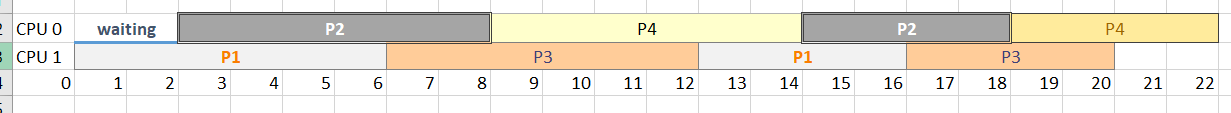
\includegraphics[width=\textwidth]{TEST2.PNG}
	    \caption{Gantt chart for processes in test os\_0}
	    \label{fig:my_label}
	\end{figure}

	\begin{lstlisting}
	# MEM status after doing allocation and deallocation of processes
    	MEMORY CONTENT: 
    000: 00000-003ff - PID: 03 (idx 000, nxt: 001)
    001: 00400-007ff - PID: 03 (idx 001, nxt: 002)
    002: 00800-00bff - PID: 03 (idx 002, nxt: 003)
    003: 00c00-00fff - PID: 03 (idx 003, nxt: -01)
    004: 01000-013ff - PID: 04 (idx 000, nxt: 005)
    005: 01400-017ff - PID: 04 (idx 001, nxt: 006)
    006: 01800-01bff - PID: 04 (idx 002, nxt: 012)
    007: 01c00-01fff - PID: 02 (idx 000, nxt: 008)
    008: 02000-023ff - PID: 02 (idx 001, nxt: 009)
    009: 02400-027ff - PID: 02 (idx 002, nxt: 010)
    	025e7: 0a
    010: 02800-02bff - PID: 02 (idx 003, nxt: 011)
    011: 02c00-02fff - PID: 02 (idx 004, nxt: -01)
    012: 03000-033ff - PID: 04 (idx 003, nxt: -01)
    014: 03800-03bff - PID: 03 (idx 000, nxt: 015)
    015: 03c00-03fff - PID: 03 (idx 001, nxt: 016)
    016: 04000-043ff - PID: 03 (idx 002, nxt: 017)
    	041e7: 0a
    017: 04400-047ff - PID: 03 (idx 003, nxt: 018)
    018: 04800-04bff - PID: 03 (idx 004, nxt: -01)
    023: 05c00-05fff - PID: 02 (idx 000, nxt: 024)
    024: 06000-063ff - PID: 02 (idx 001, nxt: 025)
    025: 06400-067ff - PID: 02 (idx 002, nxt: 026)
    026: 06800-06bff - PID: 02 (idx 003, nxt: -01)
    047: 0bc00-0bfff - PID: 01 (idx 000, nxt: -01)
    	0bc14: 64
    057: 0e400-0e7ff - PID: 04 (idx 000, nxt: 058)
    058: 0e800-0ebff - PID: 04 (idx 001, nxt: 059)
    059: 0ec00-0efff - PID: 04 (idx 002, nxt: 060)
    	0ede7: 0a
    060: 0f000-0f3ff - PID: 04 (idx 003, nxt: 061)
    061: 0f400-0f7ff - PID: 04 (idx 004, nxt: -01)
    NOTE: Read file output/os_0 to verify your result
	\end{lstlisting}
\testbf{TEST \texttt{os\_1}}
    \begin{figure}[h]
	    \centering
	    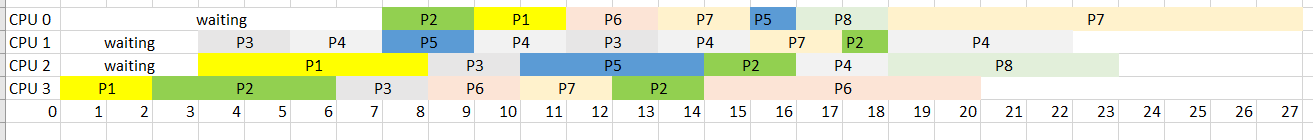
\includegraphics[width=\textwidth]{TEST3.PNG}
	    \caption{Gantt chart for processes in test os\_1}
	    \label{fig:my_label}
	\end{figure}
	\begin{lstlisting}
	# MEM status after doing allocation and deallocation of processes
    	MEMORY CONTENT: 
    000: 00000-003ff - PID: 05 (idx 000, nxt: 001)
    001: 00400-007ff - PID: 05 (idx 001, nxt: 002)
    002: 00800-00bff - PID: 05 (idx 002, nxt: 003)
    003: 00c00-00fff - PID: 05 (idx 003, nxt: 004)
    004: 01000-013ff - PID: 05 (idx 004, nxt: -01)
    009: 02400-027ff - PID: 06 (idx 000, nxt: 010)
    010: 02800-02bff - PID: 06 (idx 001, nxt: 011)
    011: 02c00-02fff - PID: 06 (idx 002, nxt: 012)
    012: 03000-033ff - PID: 06 (idx 003, nxt: -01)
    019: 04c00-04fff - PID: 01 (idx 000, nxt: -01)
    	04c14: 64
    024: 06000-063ff - PID: 05 (idx 000, nxt: 025)
    	06014: 66
    025: 06400-067ff - PID: 05 (idx 001, nxt: -01)
    031: 07c00-07fff - PID: 06 (idx 000, nxt: 032)
    032: 08000-083ff - PID: 06 (idx 001, nxt: 033)
    033: 08400-087ff - PID: 06 (idx 002, nxt: 034)
    	085e7: 0a
    034: 08800-08bff - PID: 06 (idx 003, nxt: 035)
    035: 08c00-08fff - PID: 06 (idx 004, nxt: -01)
    052: 0d000-0d3ff - PID: 05 (idx 000, nxt: 053)
    	0d3e8: 15
    053: 0d400-0d7ff - PID: 05 (idx 001, nxt: -01)
	\end{lstlisting}
	\newpage 
\begin{appendix}
  \listoffigures
\end{appendix}

\begin{thebibliography}{80}


\bibitem{bib1}
...


\bibitem{bib2}
...


\end{thebibliography}
\end{document}

